\documentclass{article}


\usepackage[utf8]{inputenc}
\usepackage[english]{babel}
\usepackage{authblk,url}
\usepackage{amssymb,amsmath,amsthm,twoopt,xargs,mathtools}
\usepackage{times,ifthen}
\usepackage{fancyhdr,xcolor}

\title{}
\date{}

%\author[$\wr$]{Mathis Chagneux}
\author[$\dag$]{XXX}
%\affil[$\wr$]{{\small LTCI, T\'el\'ecom Paris, Institut Polytechnique de Paris, Palaiseau.}}

\affil[$\dag$]{{\small CMAP, \'Ecole Polytechnique, Institut Polytechnique de Paris, Palaiseau.}}

\lhead{}
\rhead{}

\DeclareUnicodeCharacter{2212}{-}
\usepackage{geometry}
\pagestyle{fancy}

\def\dimX{d}
\def\dimY{m}
%\def\Xset{\mathsf{X}}
\def\Xset{\mathbb{R}^d}
\def\Yset{\mathsf{Y}}
\newcommand{\mk}{\kernel{G}}
\newcommand{\hk}{\kernel{Q}}
\newcommand{\md}[1]{g_{#1}}
\newcommand{\SmoothFigSize}{0.27}

\newcommand{\logllh}[1]{\ell_{#1}}
\newcommand{\llh}[1]{\mathsf{L}_{#1}}
\newcommand{\testf}{\mathsf{h}}

\newcommandx\filtderiv[2][1=]{
\ifthenelse{\equal{#1}{}}
	{\eta_{#2}}
	{\eta_{#2}^\N}
}
\newcommand{\pred}[1]{\pi_{#1}}
\newcommand{\parvec}{\theta}
\newcommand{\parspace}{\Theta}
\newcommand{\tstatletter}{\kernel{T}}
\newcommand{\retrok}{\kernel{D}}
\newcommandx\tstat[2][1=]{
\ifthenelse{\equal{#1}{}}
	{\tstatletter_{#2}}
	{\tau_{#2}^{#1}}
}
\newcommandx\tstathat[2][1=]{
\ifthenelse{\equal{#1}{}}
	{\tstatletter_{#2}}
	{\widehat{\tau}_{#2}^{#1}}
}
\newcommand{\af}[1]{h_{#1}}
\newcommand{\deriv}{\nabla_{\parvec}}

\newcommand{\kernel}[1]{\mathbf{#1}}
\newcommand{\bmf}[1]{\set{F}(#1)}
\newcommand{\set}[1]{\mathsf{#1}}

\newcommandx{\bk}[2][1=]{
\ifthenelse{\equal{#1}{}}
{\overleftarrow{\kernel{Q}}_{#2}}
{\overleftarrow{\kernel{Q}}_{#2}^{#1}}
}

\newcommandx{\bkhat}[2][1=]{
\ifthenelse{\equal{#1}{}}
{\widehat{\kernel{Q}}_{#2}}
{\widehat{\kernel{Q}}_{#2}^{#1}}
}

\newcommand{\lk}{\kernel{L}}
\newcommand{\idop}{\operatorname{id}}
\newcommand{\hd}[1]{q_{#1}}
\newcommand{\hdhat}[1]{\widehat{q}_{#1}}


\newcommand{\addf}[1]{\termletter_{#1}}
\newcommand{\addfc}[1]{\underline{\termletter}_{#1}}
\newcommand{\adds}[1]{\af{#1}}
\newcommand{\term}[1]{\termletter_{#1}}
\newcommand{\termletter}{\tilde{h}}
\newcommand{\N}{N}
\newcommand{\partpred}[1]{\pi_{#1}^\N}
\newcommand{\tstattil}[2]{\tilde{\tau}_{#2}^{#1}}
\newcommandx{\K}[1][1=]{
\ifthenelse{\equal{#1}{}}{{\kletter}}{{\widetilde{\N}^{#1}}}}
\newcommand{\hkup}{\bar{\varepsilon}}
\newcommand{\bi}[3]{J_{#1}^{(#2, #3)}}
\newcommand{\bihat}[3]{\widehat{J}_{#1}^{(#2, #3)}}

\newcommand{\kletter}{\widetilde{\N}}

\def\sigmaX{\mathcal{X}}
\def\sigmaY{\mathcal{Y}}
\def\1{\mathds{1}}
\def\pE{\mathbb{E}}
\def\pP{\mathbb{P}}
\def\plim{\overset{\pP}{\longrightarrow}}
\def\dlim{\Longrightarrow}
\def\gauss{\mathcal{N}}


\newcommand{\esssup}[2][]
{\ifthenelse{\equal{#1}{}}{\left\| #2 \right\|_\infty}{\left\| #2 \right\|^2_{\infty}}}


\newcommand{\swght}[2]{\ensuremath{\omega_{#1}^{#2}}}

\newtheorem{assumptionA}{\textbf{A}\hspace{-3pt}}
\newcommand{\rset}{\ensuremath{\mathbb{R}}}
\newcommand{\iid}{i.i.d.}

\newcommand{\smwght}[3]{\tilde{\omega}_{#1|#2}^{#3}}
\newcommand{\smwghtfunc}[2]{\tilde{\omega}_{#1|#2}}

\newcommand{\smpart}[3]{\ensuremath{\tilde{\xi}_{#1|#2}^{#3}}}
\def\aux{{\scriptstyle{\mathrm{aux}}}}
\newcommand{\bdm}{\mathsf{TwoFilt}_{bdm}}
\newcommand{\fwt}{\mathsf{TwoFilt}_{fwt}}

\newcommand{\kiss}[3][]
{\ifthenelse{\equal{#1}{}}{r_{#2|#3}}
{\ifthenelse{\equal{#1}{fully}}{r^{\star}_{#2|#3}}
{\ifthenelse{\equal{#1}{smooth}}{\tilde{r}_{#2|#3}}{\mathrm{erreur}}}}}

\newcommand{\chunk}[4][]%
{\ifthenelse{\equal{#1}{}}{\ensuremath{{#2}_{#3:#4}}}{\ensuremath{#2^#1}_{#3:#4}}
}

\newcommand{\kissforward}[3][]
{\ifthenelse{\equal{#1}{}}{p_{#2}}
{\ifthenelse{\equal{#1}{fully}}{p^{\star}_{#2}}
{\ifthenelse{\equal{#1}{smooth}}{\tilde{r}_{#2}}{\mathrm{erreur}}}}}

\newcommand{\instrpostaux}[1]{\ensuremath{\upsilon_{#1}}}
\newcommandx\post[2][1=]{
\ifthenelse{\equal{#1}{}}
	{\phi_{#2}}
	{\phi_{#2}^\N}
}

\newcommandx\posthat[2][1=]{
\ifthenelse{\equal{#1}{}}
	{\widehat{\phi}_{#2}}
	{\widehat{\phi}_{#2}^\N}
}

\newcommand{\adjfunc}[4][]
{\ifthenelse{\equal{#1}{}}{\ifthenelse{\equal{#4}{}}{\vartheta_{#2|#3}}{\vartheta_{#2|#3}(#4)}}
{\ifthenelse{\equal{#1}{smooth}}{\ifthenelse{\equal{#4}{}}{\tilde{\vartheta}_{#2|#3}}{\tilde{\vartheta}_{#2|#3}(#4)}}
{\ifthenelse{\equal{#1}{fully}}{\ifthenelse{\equal{#4}{}}{\vartheta^\star_{#2|#3}}{\vartheta^\star_{#2|#3}(#4)}}{\mathrm{erreur}}}}}

\newcommand{\XinitIS}[2][]
{\ifthenelse{\equal{#1}{}}{\ensuremath{\rho_{#2}}}{\ensuremath{\check{\rho}_{#2}}}}
\newcommand{\adjfuncforward}[1]{\vartheta_{#1}}
\newcommand{\rmd}{\ensuremath{\mathrm{d}}}
\newcommand{\eqdef}{\ensuremath{:=}}
\newcommand{\eqsp}{\;}
\newcommand{\ewght}[2]{\ensuremath{\omega_{#1}^{#2}}}
\newcommand{\ewghthat}[2]{\ensuremath{\widehat{\omega}_{#1}^{#2}}}
\newcommand{\epart}[2]{\ensuremath{\xi_{#1}^{#2}}}
\newcommand{\filt}[2][]%
{%
\ifthenelse{\equal{#1}{}}{\ensuremath{\phi_{#2}}}{\ensuremath{\phi_{#1,#2}}}%
}
\newcommand{\Xinit}{\ensuremath{\chi}}
\newcommand{\sumwght}[2][]{%
\ifthenelse{\equal{#1}{}}{\ensuremath{\Omega_{#2}}}{\ensuremath{\Omega_{#2}^{(#1)}}}}
\newcommand{\sumwghthat}[2][]{%
\ifthenelse{\equal{#1}{}}{\ensuremath{\widehat{\Omega}_{#2}}}{\ensuremath{\widehat{\Omega}_{#2}^{(#1)}}}}

\newcounter{hypH}
\newenvironment{hypH}{\refstepcounter{hypH}\begin{itemize}
\item[{\bf H\arabic{hypH}}]}{\end{itemize}}

\newcommand{\marginalset}{\mathsf{U}}

\newcommand{\calF}[2]{\mathcal{F}_{#1}^{#2}}
\newcommand{\calG}[2]{\mathcal{G}_{#1}^{#2}}
\newcommand{\Uset}{\mathsf{U}}
\newcommand{\tcalF}[2]{\widetilde{\mathcal{F}}_{#1}^{#2}}
\newcommand{\tcalG}[2]{\widetilde{\mathcal{G}}_{#1}^{#2}}

\newcommand{\kernelmarg}{\mathbf{R}}

\newcommand{\pplim}{\overset{\pP}{ \underset{\N \to \infty}{\longrightarrow}}}
\newcommand{\ddlim}{\overset{\mathcal{D}}{ \underset{\N \to \infty}{\longrightarrow}}}
\newcommand{\aslim}{\overset{\pP\mathrm{-a.s.}}{ \underset{\N \to \infty}{\longrightarrow}}}

\newcommand{\qg}[1]{\ell_{#1}}
\newcommand{\hatqg}[1]{\mathsf{\ell}_{#1}}

\newcommand{\sfd}{\mathsf{d}}
\newcommand{\X}{\mathbf{X}}
\newcommand{\x}{\mathbf{x}}
\newcommand{\y}{\mathbf{y}}
\newcommand{\E}{\mathbf{E}}
\newcommand{\e}{\text{e}}
\newcommand{\W}{\mathbf{W}}
\newcommand{\Z}{\mathbf{Z}}
\newcommand{\frob}{:}
\newcommand{\rme}{\mathrm{e}}
\newcommand{\vois}{\mathcal{V}}

\begin{document}

\maketitle

\begin{abstract}

\end{abstract}


\subsection*{First Experiments}
First experiments were focused on baselines on images and a few timeseries \footnote{List of experiments \& datasets to validate the new approach and compare to vq-vae \url{https://docs.google.com/document/d/1a7lhplsBraTD3qmvsHXdoPmQj00YijT2XMWpHEFeb58/edit}}.

\begin{itemize}
	\item \textbf{Datasets} implemented: MNIST, FashionMNIST, Cifar-10, (timeseries) Weather and Air quality
	\item \textbf{Baselines and architectures} Simple VAE model, with Feedforward, convolutional (simple) and ResNet encoder / Decoder; IWAE ; VQ-VAE, with standard implementation (straight-through gradient passing over the codebook), including the exponential moving average trick to stabilize the training of the codebook. \\
	A pixelCNN (pixelSnail) autoregressive \textit{prior} model, to learn the unconditionnal marginalized $q(z_q)$ by encoding the full dataset using the encoder.\\
	VQ-VAE with Gumbel-softmax trick, which alleviates the need for other gradient copying tricks and unstabilities (very used in VQ-VAE implementations)\\
	the Sequential mixture VQ-VAE, as described below.
  \item \textbf{Metrics} implemented: NLL on valset, Bits per dim ; FID score (pictures only) ; Inception Score (pictures only, in progress).
\end{itemize}

The sequential mixture VAE has only been tested on image generation for now. In first experiments, it achieves slightly worse scores than the standard VQ-VAE on FashionMNIST (the NLL of seqVQVAE is $0.1$ worse than VQ-VAE). The following figures show the first reconstructions. However, we did not tune the hyperparameters or the model heavily, as the sequential model does not naturally fit very well the image generation problem (it would be better on sequential data).

\begin{figure}[htp]
    \begin{center}
    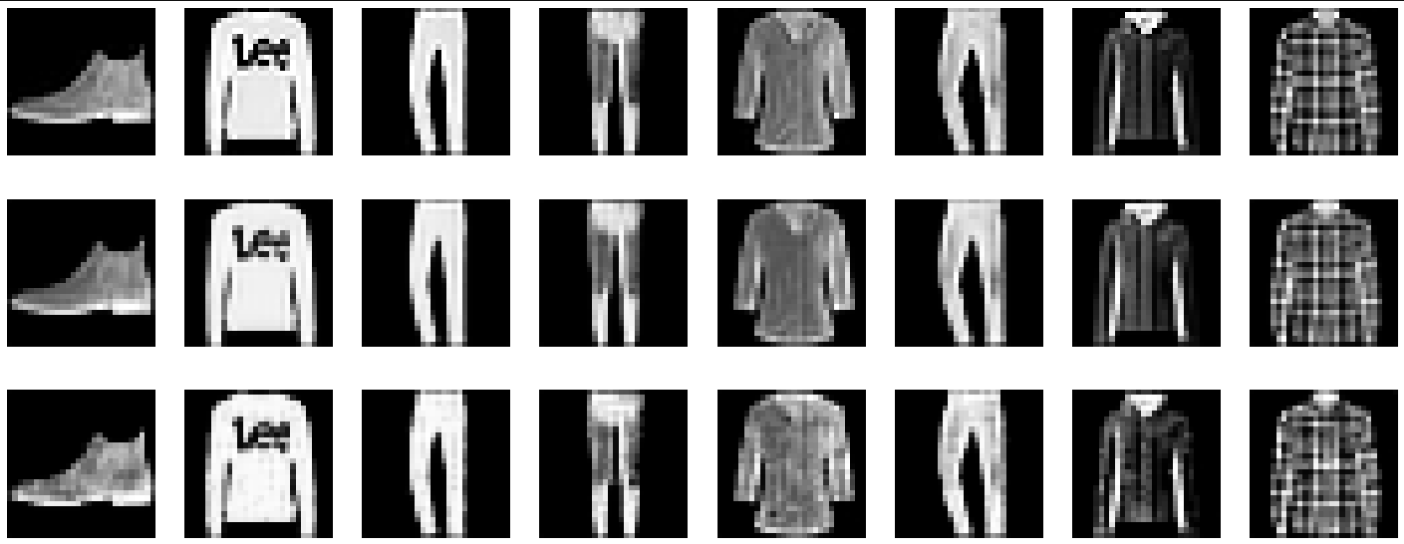
\includegraphics[width=0.37\textwidth]{images/seqvae3.png}
    \caption{FashionMNIST first reconstruction experiments. Top to bottom: originals, Reconstructions of VQ-VAE, Reconstructions of SeqVAE}
    \end{center}
\end{figure}

\begin{figure}[htp]
    \begin{center}
    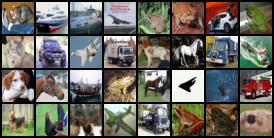
\includegraphics[width=0.37\textwidth]{images/originals.png} \\
		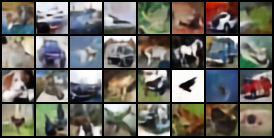
\includegraphics[width=0.37\textwidth]{images/vqvae2.png} \\
		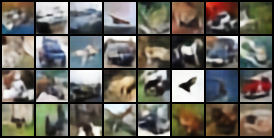
\includegraphics[width=0.37\textwidth]{images/seqvqvae2.png}
    \caption{Cifar first reconstruction experiments. Top to bottom: originals, Reconstructions of VQ-VAE, Reconstructions of SeqVAE}
    \end{center}
\end{figure}


\clearpage
\newpage

\subsection*{Mixture vq-vae}
 Let $(X^1,\ldots,X^n)$ be the observations in $\rset^D$ (a sequence of structured data, not necessarily some time series).  It is assumed that the distribution of $X$ depends on a hidden sequence of discrete states $(z_q^1,\ldots, z_q^n)$ taking values in $\{1,\ldots,K\}$ through  embedding vectors $(\rme^1,\ldots,\rme^K)$ in $\rset^m$.

\paragraph{Decoder i.e. generative model - mixture vq-vae.}
Following the standard vq-vae approach, during training it is assumed that the prior distribution of the hidden states is uniform on $\{1 \cdots K\}$. %$p_\theta(z_q)$ is uniform (i.e. we do not estimate the prior during this training phase).
%$$
%p_\theta(z_q) = \prod_{j=1}^m p(z_q^j)\eqsp,
%$$
%where $p$ is the uniform distribution on $\{1 \cdots K\}$.
Then, consider the following model:
$$
p_{\theta}(X|z_q) = \prod_{j=1}^n p_{\theta}(X^j|\vois(z_q^j)) = \varphi_{\mu_\theta(\bar e^j),\Sigma_\theta(\bar e^j)}(X)\eqsp,
$$
where $\vois(z_q^j)$ are the vectors in a neighborhood of  $z_q^j$, $\bar e^j = \{e^{z_q^\ell}\;;\; z_q^\ell\in \vois(z_q^j)\}$ and where $\varphi_{\mu,\sigma}$ is the Gaussian probability density function with mean $\mu$ and variance matrix $\Sigma$. We may consider for instance $\vois(z_q^j) = \{z_q^{j-p} \cdots z_q^j\}$.

\paragraph{Encoder - mixture vq-vae.} Consider an encoding function $f_\theta$ and write
$$
(z_\rme^1,\ldots, z_\rme^m) = f_\eta(X^{1:n})\eqsp.
$$
Note that the function $f_\eta$ does not build as many encoding states $(z_\rme^1,\ldots, z_\rme^m)$ as the number of observations.
%The parameters $\theta$ are estimated through gradient descent during the training.

\paragraph{Quantization} Consider a variational family $q_\varphi(z_q^{1:m}|z_e^{1:m})$ given by a recurrent neural network. Set $h^0 = 0$, and for all $1 \leq j \leq m$ and all $1 \leq k \leq K$,
\begin{align*}
    h^j &= \tanh(W_z z_e^j + W_h h^{j-1} + b)\,, \\
    p^j &= \texttt{softmax}\left(\left\{- \| \rme_k - h^j\|^2\right\}_{1\leqslant k \leqslant K}\right)\,,
\end{align*}
where $W_z, W_h$ and $b$ are the unknownweight matrices and vector of the neural network.
%In the specific conditions where $W_z = I_d$ and $W_h = b = 0$, these equations lead to
%$$
%p^j_k = \texttt{softmax}(- \| \rme_k - \tanh(z_e^j) \|^2)\,.
%$$
Codebook vectors are sampled  from the categorical distribution based on the computed $p^j_{1:K}$:
$$
q_\varphi(z_q^{1:m} | z_e^{1:m}) = \prod_{j=1}^m p_\theta(z_q^j|z_e^{1:j}) = \prod_{j=1}^m \texttt{Cat}(\{p^j_k\}_{k=1}^K)\,.
$$
During training, we replace the categorical distribution by a Gumbel distribution, in order to define a differentiable quantization.

\paragraph{Training}
We minimize the loss
$$
\mathcal{L}(\theta, \varphi) = \mathbb{E}_{q_\varphi} \left[ \log\left(\frac{p_\theta(x|z_q)}{q_\varphi(z_q|z_e)}\right) \right]
$$
If we consider $\Sigma_\theta$ to be a diagonal matrix, with values $\Sigma_\theta = \texttt{diag}(\{\sigma_{\theta, i}^2\}_{i=1}^d)$:
\begin{align*}
    \log p_\theta(x|z_q^j) &= \log \varphi_{\mu_\theta(\vois(z_q^j)),\Sigma_\theta(\vois(z_q^j))}(x) \\
			   &= \log\left(|\Sigma_\theta(\vois(z_q^j))|^{-\frac{1}{2}} \exp\left(-\frac{1}{2}(x - \mu_\theta(\vois(z_q^j)))^T \Sigma_\theta(\vois(z_q^j))^{-1} (x - \mu_\theta(\vois(z_q^j))) \right)\right) \\
			   &= -\sum_{i=1}^d \log(\sigma_{\theta, i}(\vois(z_q^j))) -\frac{1}{2} \sum_{i=1}^d \frac{(x_i - \mu_\theta(\vois(z_q^j)))^2}{\sigma_{\theta, i}^2(\vois(z_q^j))}
\end{align*}
where constant terms have been omitted.

\paragraph{Sequential data case}
In the case of sequential data, we may consider the model
$$
p_{\theta}(X|z_q) = \prod_{j=1}^n p_{\theta}(X^j|\vois(z_q^j)) = \varphi_{\mu_\theta(\bar e^j),\Sigma_\theta(\bar e^j)}(X)\eqsp,
$$
Where the neighborhood $\vois(z_q^j)$ and $\bar e^j$ are defined such that a single $X^t$ only depend on a few previous corresponding $z_q^j$ (note that $t \in \rset^n$ is typically larger than $j \in \rset^m$).

\paragraph{Diffusion-based variational model suited for images and sequential data such as text}
We consider an alternative model, where we do not consider the prior uniform anymore, but rather parametrize it with a diffusion model: consider a family of progressively noised variables $Z_q^0, \cdots, Z_q^T$, where we choose $Z_q^T$ to be uniform. We consider the following model:

$$
p_{\theta}(Z_q^0, \cdots, Z_q^T, X) = p_{\theta}(z_q^T) p_{\theta}(z_q^0|z_q^1) \cdots p_{\theta}(X|z_q)
$$

where $p_{\theta}(z_q^0|z_q^1)$ is a newly parametrized denoising model, typically a deep neural network, and $p_{\theta}(X|z_q)$ is defined as in previous section. We then consider the following variational familly:

$$
q_{\varphi}(Z_q^0, \cdots, Z_q^T | X) = q_{\varphi}(Z_q^0 | X) q_{\varphi}(Z_q^1 | Z_q^0, X) \cdots
$$

Where $q_{\varphi}(Z_q^0 | X)$ is similar to previous section. Using the auxiliary variational inference framework (AVI), where $u = Z_q^{1:T}$, $x = Z_q^0$ and $z = X$, we have:
$$
\mathbb{E}_{q_\varphi (Z_q^0, Z_q^{1:T}|X)} \left[ \log\left(\frac{p_\theta(Z_q^{0:T})p_\theta(X|Z_q^0)}{q_\varphi(Z_q^0|X) q_\varphi(Z_q^{1:T}|Z_q^0)}\right) \right]
$$

\clearpage
\newpage


\paragraph{a few words on Gumbel-Softmax}
We consider a similar mixture VQ-VAE model, with same encoder and decoder. However, instead of modeling sequential dependancies in the latent space using a RNN for $q_\varphi(z_q^{1:m}|z_e^{1:m})$, we instead take inspiration from score-based diffusion models. First, as mentionned previously, recall that the categorical distribution is replaced by a Gumbel distribution:
\begin{align*}
	h_k^l &= - \| \rme_k - z_e^l\|^2\,, \\
	p_k^l &= \frac{e^{((G_k + log(h_k^l)) / \tau)}}{\sum_j e^{((G_j + log(h_j^l)) / \tau)}}\,, \\
	z_q^l &= \sum_{k=1}^K p_k^l \rme_k\,. \\
\end{align*}

where $G_k$ is a Gumbel noise, and $\tau$ a temperature ($\tau \rightarrow 0$ is similar to a hard sampling under the softmax probabilities, while $\tau \rightarrow \infty$ similar to a uniform distribution). Our intuition is that we should gradually anneal the distribution with well chosen $\tau$, to get two interesting benefits.
\begin{enumerate}
	\item a stable training, as we will explore well the different $\rme_k$ when $\tau$ is high (a common problem in VQ-VAEs), while having a good Categorical sampling approximation when $\tau$ is low.
	\item a natural way to learn a "prior" for the latent distribution, by learning to invert the annealing process.
\end{enumerate}
This motivates a "Gumbel-diffusion process".

\paragraph{a few words on Categorical Diffusion Process}
Following \url{https://arxiv.org/abs/2102.05379}, we consider the following categorical diffusion process $q_D$ (omitting $j$ index for clarity) with $\beta_t$ chance to resample a category uniformly:
\begin{align*}
	q_D(x_0) &= \texttt{Cat}(\{p_k\}_{k=1}^K)\,, \\
	q_D(x_t | x_{t−1}) &= \texttt{Cat}(x_t|(1 − \beta_t)x_{t−1} + \beta_t/K)\,, \\
	q_D(x_t|x_0) &= \texttt{Cat}(x_t|\alpha^\prime_t x_0 + (1 − \alpha^\prime_t)/K)\,.
\end{align*}

Here $\alpha_t = 1 − \beta_t$ and $\alpha^\prime_t = \prod_{t^\prime=1}^t \alpha_t^\prime$. We refer to the paper for more information (this is a draft).

With further work, it should be possible to build a noise conditional score convolutional neural network $s(x_t, \beta_t)$ which learns the score of the perturbed distribution $\nabla_{\x_t} \log q_D(x_t, \beta_t)$. We would then be able to use a langevin dynamics process making use of this score network and a random init vector $x_T$ from a uniform distribution to produce a sample $x_0^\prime$ after $T$ steps, from the "prior" distribution with the right global dependencies.

It would be interesting to relate the Gumble Softmax with this process formally, to build the complete loss function, as well as to see which steps of the diffusion process would be used to learn the encoder / decoder / codebook parameters (there are several possibilies here, 1) taking only $x_0$, 2) selecting a random step, 3) using all of them $x_0$ up to $x_T$?)
%where $\|z_\rme^{k}-\rme_i\|^2_{\Omega} = (z_\rme^{k}-\rme_i)^T\Omega (z_\rme^{k}-\rme_i)$. This mean-field variational distribution assumes that the latent $(z_q^1,\ldots, z_q^m)$ are independent given $(X^1,\ldots,X^n)$ and $(z_\rme^1,\ldots, z_\rme^m)$.
%The variational posterior can be defined as a marginal distribution, $q_\phi(z_q|x) = \int
%\bar{q}_\phi (z_q, z_\rme |x) \rmd z_\rme$, where $\bar{q}_\phi(z_q,z_\rme|x)$ has an explicit closed-form.
%The auxiliary variables $z_\rme$ lead to the objective
%\begin{equation*}
%\int \bar{q}_\phi(z_q,z_\rme
%|x) \log \left( \frac{\bar{p}_\theta(z_q,z_\rme,x)}{\bar{q}_\phi(z_q,z_\rme|x)} \right)  \rmd z_q \rmd z_\rme \eqsp.
%\end{equation*}

\clearpage
\newpage

\subsection*{Draft for the new approach}
 Let $(Y^1,\ldots,Y^n)$ be the observations in $\rset^q$ (a sequence of structured data, not necessarily some time series).
\paragraph{Encoder.} Consider an encoding function $f_\theta$ (proper neural network-based encoder  to be defined when the model is fixed) and write
$$
(z_\rme^1,\ldots, z_\rme^m) = f_\theta(Y^{1:n})\eqsp.
$$
Note that the function $f_\theta$ does not build as many encoding states $(z_\rme^1,\ldots, z_\rme^m)$ as the number of observations.
In the initial approach \textcolor{red}{we keep the exact same $f_{\theta}$ and therefore the same $(z_\rme^1,\ldots, z_\rme^m)$ than in the original vq-vae.}
We propose then to introduce a variational family to model the conditional distribution of $(z_q^1,\ldots, z_q^m)$ given $(Y^1,\ldots,Y^n)$.
$$
q_\varphi (z_q^{1:m} |Y^{1:n}) = q_\varphi(z_q^{1}|Y^{1:n})\prod_{k=1}^m q_\varphi(z_q^{k+1}|z_q^{k},Y^{1:n}) \eqsp,
$$
where the initial distriubtion and the transition kernel depend on $(z_\rme^1,\ldots, z_\rme^m)$.

\paragraph{Decoder.} For the initial approach we use the same decoder as in the original vq-vae $p_{\theta}(Y^{1:n}|z_q^{1:m})$.

\paragraph{ELBO 1.}
The loss function is of the form
$$
\mathcal{L}(\theta,\varphi) = \mathbb{E}_{q_\phi}\left[\log\frac{p_\theta(z_q^{1:m},Y^{1:n})}{q_\varphi(z_q^{1:m}|Y^{1:n})}\right]
$$
Here, samples from $\mathcal{L}(\theta,\varphi)$ are obtained easily (VAE or IWAE style). In the first approach we want to see the impact of the choice of $q_\phi$ so that $p_\theta(z_q^{1:m})$ is chosen as the uniform distribution.
We can then compare the original vq-vae with this version.

\paragraph{ELBO 2.}
We can also propose a model for $p_\theta(z_q^{1:m})$.
\begin{enumerate}
\item We can use a complex fully-parameterized model $p_\theta(z_q^{1:m})$.
\item Or we can use another mini-bacth of observations to sample many $z_q^{1:m}\sim \frac{1}{M}\sum_{i=1}^M q_\varphi(\cdot | Y^{1:n})$.
\end{enumerate}
$$
\mathcal{L}(\theta,\varphi) = \mathbb{E}_{q_\phi}\left[\log\frac{p_\theta(z_q^{1:m},Y^{1:n})}{q_\varphi(z_q^{1:m}|Y^{1:n})}\right]
$$
Here, samples from $\mathcal{L}(\theta,\varphi)$ are obtained easily (VAE or IWAE style).

\paragraph{Implementation considerations}
(draft) We consider the case described in ELBO 1. From a batch of observations $Y$ compute the $z_e^{1:m} = f_{\theta}(Y^{1:n})$, where $f_{\theta}$ is a typical encoder. The following options can be explored to compute the $z_q^{1:m}$ from the $e_j$ and $z_e^{1:m}$.
\begin{enumerate}
\item (vqvae: all independant, no model) $z_q^{i} = e_j$ where $j = argmin_j ||z_e^i - e_j||^2$.
\item (mixture vqvae: all independant) $q_\varphi(z_q^{i}|z_e^{i})$ is a mixture of the code vectors $e_j$ (see below).
\item (adding a Markov structure) $q_\varphi(z_q^{1}|z_e^{1})$ is a mixture of the code vectors $e_j$, then $q_\varphi(z_q^{k+1}|z_q^{k},z_e^{k+1})$ is described below.
\item (full parametrized model (ELBO 2.)): $q_\varphi(z_q^{1:m}|z_e^{1:m}, e_j)$: unclear how to do it, and probably complex to learn efficiently. A possibility using the original VQ-VAE pixelCNN, i.e. an autoregressive model is described below
\item (iterative model (ELBO 2.)): Would it be possible to build an iterative estimate of $z_q^{1:m}$ by first considering them independant, then using a parametrized model to refine them depeding on their local dependency (like a diffusion model https://arxiv.org/abs/2006.11239)
\end{enumerate}

Mixture for a single element (2):
$$w_j^{i} = ||e_j - z_e^{i}||$$
$$q_\varphi(z_q^{i}|z_e^{i}) = q^\star_\varphi(z_q^{i}|z_e^{i}) = softmax(\frac{\mathbf{w}^{i}}{\tau})$$


Mixture with markov structure (3):
$$q_\varphi(z_q^{1}|z_e^{1}) = q^\star_\varphi(z_q^{1}|z_e^{1})$$
$$Q_{\theta} = g_{\theta}(Y^{1:n})$$
$$q_\varphi(z_q^{k+1}|z_q^{k},z_e^{k+1}) = (q^\star_\varphi(z_q^{i}|z_e^{i}))^\alpha \times (Q_{\theta} \cdot z_q^{k})^{(1 - \alpha)}$$
where $g_{\theta}$ has shared parameters with the encoder (typically a second encoder head), and $Q_{\theta}$ is a transition matrix of size $K \times K$ (parametrization to be defined, take inspiration from attention models). $\alpha$ could be parametrized as well, depending on whether we matched well $z_e^i$ to a codebook vector $e_j$ (i.e. depeding on the  $min_j||e_j - z_e^{i}||$)

Mixture with an autoregressive model (4) $g_{\theta}$ is typically a RNN, PixelCNN, WaveNet:
$$q_\varphi(z_q^{1}|z_e^{1}) = q^\star_\varphi(z_q^{1}|z_e^{1})$$
$$q_\varphi(z_q^{k+1}|z_q^{1:k},z_e^{k+1}) = O(g_{\theta}(z_q^{1:k}), q^\star_\varphi(z_q^{k+1}|z_e^{k+1}))$$

Where $O$ is a mixing function, enabling to select whether we should take the input from the autoregressive model or from the input (could be similar to previous).


Finally, regardless of the model, we can get the $z_q^{i}$ vector as such
$$ z_q^{i} = \sum_j^m q_\varphi(z_q^{i}|\cdot)_j e_j$$

\clearpage
\newpage

\paragraph{Discrete latent states.} The crucial step to estimate the parameter is to compute
$$
\nabla_\theta\mathcal{L}(\theta) = \nabla_\theta \mathbb{E}_{\hat{\theta}_p}\left[\log p_{\theta}(z^{1:m}_q,Y^{1:n})  \middle | Y^{1:n}\right]\eqsp,
$$
i.e. to compute an expectation under the distribution of the sequence $z^{1:m}_q$ given the observations $Y^{1:n}$. Following the original vq-vae, we then propose a model for the conditional distribution of the sequence $z^{1:m}_q$ given $Y^{1:n}$ (and not for the prior distribution of the discrete states). Consider $(\rme^1,\ldots,\rme^K)$ the K embedding vectors. Let $Y^{-k}$ be observations in a neighborhood of $Y^k$. From $(z_\rme^1,\ldots, z_\rme^m)$ and the observations, the model builds a Markov chain (we may consider more comple dependencies) $(z_q^1,\ldots, z_q^n)$ taking values in $\{\rme^1,\ldots,\rme^K\}$ such that:
$$
\mathbb{P}_\theta(z_q^1 = \rme^j|Y^{1:n}) = \mu_\theta[z_\rme^1,Y^{-1}](\rme^j) \eqsp,\quad \mathbb{P}_\theta(z_q^{k+1} = \rme^j | z_q^{k} =  \rme^\ell,Y^{1:n}) = Q_{\theta}[z_\rme^{k},z_\rme^{k+1},Y^{-k}](\rme^\ell,\rme^j)\eqsp,
$$
where, for all $z,z'$, $\{\mu_{\theta}[z,Y^{-1}](\rme^j)\}_{1\leqslant j\leqslant K}$ is a probability vector and $\{Q_{\theta}[z,z',Y^{-k}](\rme^\ell,\rme^j)\}_{1\leqslant j,\ell\leqslant K}$ is a transition matrix on $\{\rme^1,\ldots, \rme^K\}$.
\paragraph{Decoder.} The conditional law of the observation $Y_{k}$ given $\mathcal{F}_k$ (proper $\sigma$-field to be defined when the model is fixed, a neihnorhood of observations and latent states) is written
$$
Y^{k} = \mu^{z_q^{k}}_\theta(Y^{-k}) + \sigma^{z_q^{k}}_\theta(Y^{-k})\varepsilon_{k}\eqsp,
$$
where the $\{\varepsilon_{k}\}_{1\leqslant k\leqslant n}$ are i.i.d. standard Gaussian random variables in $\rset^q$ and $(\mu^{j},\sigma^{j}_\theta)$ are outputs of some neural network architecture to be defined  (proper neural network-based encoder  to be defined when the model is fixed). \textcolor{red}{The observation model for $Y^k$ may depend on more latent state than $z_q^k$.}
\paragraph{Training.}
The gradient step is given by
\begin{multline*}
\nabla_\theta\mathcal{L}(\theta) = \nabla_\theta \mathbb{E}_{\hat{\theta}_p}\left[\log p_{\theta}(z^{1:m}_q,Y^{1:n})  \middle | Y^{1:n}\right] \\
=  \nabla_\theta \mathbb{E}_{\hat{\theta}_p}\left[\log p_{\theta}(z^{1:m}_q)  \middle | Y^{1:n}\right]  + \nabla_\theta \mathbb{E}_{\hat{\theta}_p}\left[\log p_{\theta}(Y^{1:n}|z^{1:m}_q)  \middle | Y^{1:n}\right]\eqsp.
\end{multline*}
The second term is easy to compute (depending on the complexity of $ p_{\theta}(Y^{1:n}|z^{1:m}_q)$ but we may start with something easy) as the computational expecation is computed with the conditional kernel. The second term is trickier, it is the term trained in a separate learning framework in vq-vae. We should use the explicit marginalization
$$
 p_{\theta}(z^{1:m}_q) \sim \int p_{\theta}(z^{1:m}_q|y^{1:n})p_*(\rmd y^{1:n})
$$
and provide a Monte Carlo estimate based on samples from $p_\star$, i.e. samples from the dataset.



\clearpage
\newpage
\textcolor{red}{The notes below are not useful anymore... for now!}


\section{Introduction}
\label{sec:intro}

\section{Mixture-based vq-vae}
\label{sec:model:mixture}
\subsection{Model and architectures}
Let $X_I \in \rset^d$ be the input data and $Y$ be the observations in $\rset^q$.  Several frameworks.

\paragraph{Encoder.} Consider an encoding function $f_\theta: \rset^d \to \rset^{m}$ (proper neural network-based encoder  to be defined when the model is fixed) and write
$$
z_\rme = f_\theta(X_I)\eqsp.
$$


\paragraph{Discrete latent states.} Consider $(\rme^1,\ldots,\rme^K)$ the K embedding vectors in $\rset^m$. From $z_\rme$ the model builds a latent state $z_q$ taking values in $\{\rme^1,\ldots,\rme^K\}$ such that:%(this set is identified with $\{1,\ldots, K\}$ in throughout the paper)
$$
\mathbb{P}_\theta(z_q= \rme^j) = \rho^{}_{\theta}(z_\rme;\rme^j) \eqsp,
$$
where, for all $z\in\rset^m$, $\{\rho_{\theta}(z;\rme^j)\}_{1\leqslant j\leqslant K}$ is a probability vector on  $\{\rme^1,\ldots,\rme^K\}$.
\paragraph{Decoder.} The conditional law of the observation $Y$ given $\mathcal{F}$ (proper $\sigma$-field to be defined when the model is fixed) is written
$$
Y = \mu_\theta(z_q) + \sigma_\theta(z_q)\varepsilon\eqsp,
$$
where the $\varepsilon$ is a standard Gaussian random variables in $\rset^q$ and for all $z\in\rset^m$, $\{\mu_\theta(z),\sigma_\theta(z)\}$ are outputs of some neural network architecture to be defined  (proper neural network-based encoder  to be defined when the model is fixed).

\subsection{Loss function}
The (complete) loglikelihood of the model (conditionally on $X_I$ which is dropped from the notations) is given by
$$
\log p_{\theta}(z_q,Y) =  \log \rho^{}_{\theta}(z_\rme;z_q) +  \log \varphi_{\mu^{}_\theta (z_q),\sigma^{}_\theta (z_q)}(Y) \eqsp,
$$
where $\varphi_{\mu,\sigma}$ is the Gaussian probability density function with mean $\mu$ and variance $\sigma^2$. The posterior distribution of $z_q$ given $Y$ is
$$
\mathbb{P}_\theta(z_q = \rme^j|Y) = \frac{\rho^{}_{\theta}(z_\rme;\rme^j)\varphi_{\mu_\theta(\rme^j),\sigma^{}_\theta(\rme^j)}(Y)}{\sum_{k=1}^{K}\rho^{}_{\theta}(z_\rme;\rme^k)\varphi_{\mu_\theta(\rme^k),\sigma_\theta(\rme^k)}(Y)} = \omega^j_{z}\eqsp.
$$
Then, consider the loss function (Fisher or EM based update),
$$
\mathcal{L}(\theta) = \mathbb{E}\left[\log p_{\theta}(z_q,Y)  \middle | Y\right] = \sum_{j=1}^K  \omega^j_{z}\log p_{\theta}(\rme^j,Y)=  \sum_{j=1}^K  \omega^j_{z}\left\{\log \rho^{}_{\theta}(z_\rme;\rme^j) +  \log \varphi_{\mu^{}_\theta(\rme^j),\sigma^{}_\theta(\rme^j)}(Y)\right\}\eqsp.
$$
An alternative is to compute the estimate $\mathbb{E}_\theta[z_q|Y] = \sum_{j=1}^K  \omega^j_{z}\rme^j$.

\section{Application to time series}
\label{sec:model}
Following the previous section, the crucial step to estimate the parameter is to compute
$$
\mathcal{L}(\theta) = \mathbb{E}\left[\log p_{\theta}(z^{1:n}_q,Y^{1:n})  \middle | Y^{1:n}\right]\eqsp,
$$
i.e. to compute an expectation under the distribution of the sequence $z^{1:n}_q$ given the observations $Y^{1:n}$.

In the case where $z^{1:n}_q$ is a Markov chain, we know that conditionally on $Y^{1:n}$, $z^{1:n}_q$ is a Markov chain which revolves backwards in time. Instead of computing the backward Markov kernel from the prior kernel of $z^{1:n}_q$ (see the computations below) we propose to directly model the backward Markov kernel.

For all $z\in\rset^m$, $y^{1:n}$, let $\{\mu^{z,y^{\underline\kappa(n):n}}_{\theta}(j)\}_{1\leqslant j\leqslant K}$ be a probability vector and $Q_k^{z,y^{\underline\kappa(k):\overline\kappa(k)}}$ be a transition matrix on $\{\rme^1,\ldots, \rme^K\}$. For each $k$,$\{\underline\kappa(k)\ldots,\overline\kappa(k)\}$ is the time frame around $k$ selecting the observations used as an input for  $Q_k^{z,y^{\underline\kappa(k):\overline\kappa(k)}}$.

\subsection{Model and architectures}
Let $X_I \in \rset^d$ be the input data and $(Y^1,\ldots,Y^n)$ be the observations in $\rset^q$.  Several frameworks.
\begin{enumerate}
\item $X_I$ contains weather forecasts and building management settings for the next 3 days. The observations $(Y^1,\ldots,Y^n)$  are the temperatures/energy consumptions to predict.
\item Visual language modeling.
\end{enumerate}

\paragraph{Encoder.} Consider an encoding function $f_\theta: \rset^d \to \rset^{m\times n}$ (proper neural network-based encoder  to be defined when the model is fixed) and write
$$
(z_\rme^1,\ldots, z_\rme^n) = f_\theta(X_I)\eqsp.
$$
The function $f_\theta$ builds as many encoding states $(z_\rme^1,\ldots, z_\rme^n)$ as the number of observations.

\paragraph{Discrete latent states.} Consider $(\rme^1,\ldots,\rme^K)$ the K embedding vectors in $\rset^m$. From $(z_\rme^1,\ldots, z_\rme^n)$ the model builds a Markov chain $(z_q^1,\ldots, z_q^n)$ taking values in $\{\rme^1,\ldots,\rme^K\}$ (this set is identified with $\{1,\ldots, K\}$ in the following)  such that:
$$
\mathbb{P}_\theta(z_q^1 = j) = \mu^{z_\rme^1}_{\theta}(j) \eqsp,\quad \mathbb{P}_\theta(z_q^{k+1} = j | z_q^{k} =  \ell) = Q^{z_\rme^{k+1}}_{\theta}(\ell,j)\eqsp,
$$
where, for all $z\in\rset^m$, $\{\mu^z_{\theta}(j)\}_{1\leqslant j\leqslant K}$ is a probability vector and $\{Q^{z}_{\theta}(\ell,j)\}_{1\leqslant j,\ell\leqslant K}$ is a transition matrix on $\{1,\ldots, K\}$.
\paragraph{Decoder.} The conditional law of the observation $Y_{k+1}$ given $\mathcal{F}_k$ (proper $\sigma$-field to be defined when the model is fixed) is written
$$
Y^{k+1} = \mu^{z_q^{k+1}}_\theta \!\!\!\!\!(Y^{k}) + \sigma^{z_q^{k+1}}_\theta\!\!\!\!\!(Y^{k})\varepsilon_{k+1}\eqsp,
$$
where the $\{\varepsilon_{k}\}_{1\leqslant k\leqslant n}$ are i.i.d. standard Gaussian random variables in $\rset^m$ and $(\mu^{j},\sigma^{j}_\theta)$ are outputs of some neural network architecture to be defined  (proper neural network-based encoder  to be defined when the model is fixed).

\subsection{Loss function}
The (complete) loglikelihood of the model (conditionally on $X_I$ which is dropped from the notations) is given by
\begin{align*}
\log p_{\theta}(z_q^{1:n},Y^{1:n}) =  \log \mu^{z_\rme^1}_{\theta}(z_q^1) + \sum_{k=0}^{n-1} \log  Q^{z_\rme^{k+1}}_{\theta}(z_q^k,z_q^{k+1})
+ \sum_{k=0}^{n-1} \log \varphi_{\mu^{z_q^{k+1}}_\theta\!\!\!\!\!(Y^{k}),\sigma^{z_q^{k+1}}_\theta\!\!\!\!\!(Y^{k})}(Y_{k+1}) \eqsp,
\end{align*}
where $\varphi_{\mu,\sigma}$ is the Gaussian probability density function with mean $\mu$ and variance $\sigma^2$. The posterior distribution of $(z_q,z_q^{k+1})$ given $Y^{1:n}$ is written (see computation below)
$$
\mathbb{P}_\theta(z^k_q = \rme^j,z^k_q = \rme^\ell|Y^{1:n}) =  \omega^{j,\ell}_{z,k,k+1|n}\eqsp.
$$
Then, consider the loss function (Fisher or EM based update),
\begin{align*}
\mathcal{L}(\theta) &= \mathbb{E}\left[\log p_{\theta}(z^{1:n}_q,Y^{1:n})  \middle | Y^{1:n}\right]\eqsp,\\
& =  \sum_{j=1}^K\omega^{j}_{z,1|n}\log \mu^{z_\rme^1}_{\theta}(\rme^j) + \sum_{k=0}^{n-1}\sum_{j,\ell=1}^K   \omega^{j,\ell}_{z,k,k+1|n}\left\{ \log  Q^{z_\rme^{k+1}}_{\theta}(\rme^j,\rme^\ell) +  \log \varphi_{\mu^{\rme^\ell}_\theta (Y^{k}),\sigma^{\rme^\ell}_\theta(Y^{k})}(Y_{k+1})  \right\}\eqsp,
\end{align*}
where $\omega^{j}_{1,z|n} = \sum_{\ell=1}^K\omega^{j,\ell}_{z,1,2|n}$


%
%If we use a score-based estimation procedure, the parameter update is based on
%$$
%\nabla_{\theta}\log p_{\theta,\rme^{1:n}}(Y^{1:n})\eqsp.
%$$
%An estimation of this gradient is given by
%$$
%\nabla_{\theta} \log p_{\theta,\rme^{1:n}}(\hat z_q^{1:n},Y^{1:n})\eqsp,
%$$
%where $\hat z_q^{1:n} \sim p_{\theta,\rme^{1:n}}(z_q^{1:n}|X_I,Y^{1:n})$.

\paragraph{Computation of the posterior weights}
Such a sample can be obtained with Baum-Welch algorithm.
First compute during the forward pass the discrete distributions $\phi_k$, where $\phi_k$ denotes the distribution of $z_q^k$ given $(X_I,Y^{1:k})$ as follows.
\begin{enumerate}
\item For all $1\leqslant j \leqslant K$,
$$
\phi_1(j) \propto \mu^{z_\rme^1}_{\theta}(j) \varphi_{\mu^{z_q^{1}}_\theta,\sigma^{z_q^{1}}_\theta}(Y_1)\eqsp.
$$
\item For all $1\leqslant j \leqslant K$ and  $1\leqslant k \leqslant n$,
$$
\phi_{k+1}(j) \propto \sum_{\ell=1}^K \phi_{k}(\ell)  Q^{z_\rme^{k+1}}_{\theta}(\ell,j) \varphi_{\mu^{j}_\theta (Y^{k}),\sigma^{j}_\theta(Y^{k})}(Y_{k+1})\eqsp.
$$
\end{enumerate}
Then, the weights $ \omega^{j,\ell}_{z|k,k+1}$ are computed recursively backward
%Then, to sample $\hat z_q^{1:n} \sim p_{\theta,\rme^{1:n}}(z_q^{1:n}|X_I,Y^{1:n})$, the Baum-Welch proceeds recursively backward as follows.
\begin{enumerate}
\item For all $1\leqslant \ell,j \leqslant K$,
$$
\omega^{j,\ell}_{z,n-1,n|n} \propto \phi_{n-1}(j)Q^{z_\rme^{n}}_{\theta}(j,\ell) \varphi_{\mu^{\ell}_\theta(Y^{n-1}),\sigma^{\ell}_\theta(Y^{n-1})}(Y_{n})\phi_{n}(\ell)   \eqsp.
$$
\item For all  $1\leqslant k \leqslant n-2$,
$$
\omega^{j,\ell}_{z,k,k+1|n} \propto \phi_{k}(j)Q^{z_\rme^{k+1}}_{\theta}(j,\ell) \varphi_{\mu^{\ell}_\theta(Y^{k}),\sigma^{\ell}_\theta(Y^{k})}(Y_{k+1})\omega^{\ell}_{z,k+1|n}  \eqsp,
$$
where $\omega^{\ell}_{z,k+1|n} = \sum_{m=1}^K\omega^{\ell,m}_{z,k+1,k+2|n}$.
\end{enumerate}

\subsection{Training algorithm}
%\bibliographystyle{apalike}
%\bibliography{vqvae}


\end{document}
